%++++++++++++++++++++++++++++++++++++++++
% Don't modify this section unless you know what you're doing!
\documentclass[a4paper,12pt]{article}
\usepackage{listings} % code blocks
\usepackage{tabularx} % extra features for tabular environment
\usepackage{amsmath}  % improve math presentation
\usepackage{graphicx} % takes care of graphic including machinery
\usepackage{subcaption} % necessary for subfigures
\usepackage{float}
\usepackage[margin=3.0cm,a4paper]{geometry} % decreases margins
%\usepackage{cite} % takes care of citations
%\usepackage[final]{hyperref} % adds hyper links inside the generated pdf file
%++++++++++++++++++++++++++++++++++++++++

\setlength{\parindent}{0pt}
\usepackage{hyperref}

\begin{document}

\title{Deep Learning Lab \\ Exercise 02 }
\author{Megan Klaiber}
\date{\today}
\maketitle

\section{Introduction}

In this exercise a convolutional neural network (CNN) will be implemented to classify the handwritten MNIST digits. Different hyperparameter experiments examine their influence on the network's performance.

\subsection{CNN Implementation}
The CNN structure is oriented towards LeNet. It consists of two convolutional layers with 16 3x3 filters (stride 1, same padding), each followed by a ReLU activation function and a max pooling layer of size 2. A fully connected layer succeed with 128 units and a softmax layer is used subsequent. The network is optimized with cross-entropy loss and stochastic gradient descent. Tensorflow is used for the implementation.

\section{Learning Rate}\label{lr}

The first experiment examines the bahaviour of different learning rates (lr). Therefore four different values are tested : \{0.1, 0.01, 0.001, 0.0001\} \\
\autoref{fig:lr} shows the validation error with the specified learning rates during 12 epochs. You can see that the curves differ from each other. While the error of three tested learning rates converges really fast, the one with the smallest value shrinks slowly. It is likely that this error also converges during additional training epochs. So it is very useful to try out different learning rates for faster learning.\\
It looks like the lr = 0.1 works best here because it converges quickly to the lowest error rate. Due to the high learning rate it is possible that overfitting happens. If the learning rate is too small the risk for underfitting or long converging time is increased (see lr = 0.0001).

\begin{figure}[H]
	\centering 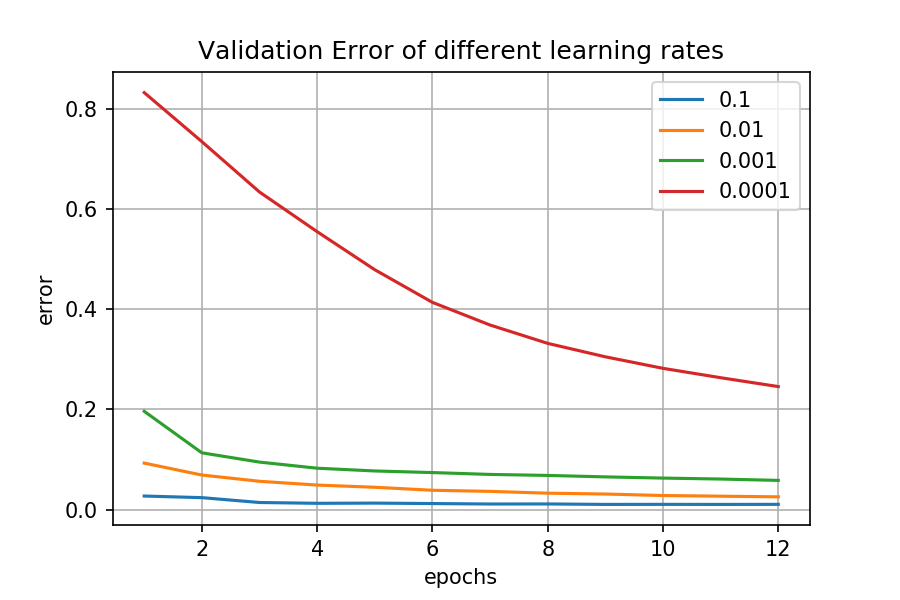
\includegraphics[width=11.70cm, height=7.9cm]{plots/lr/valid_error_12.png}
	\caption{
		\label{fig:lr}
		Change of validation error during 12 training epochs and with different learning rates.
	}
\end{figure}

\section{Convolution Type}\label{filter}

In the second experiment the filter size in the convolutional layer is evaluated. The following values are tested: \{1, 3, 5, 7\}\\
In \autoref{fig:filter} you see that the error of the smallest filter size of 1 converges slower than the others. A network with larger filters can recognize objects in images where it needs more context for a decision. In contrast to that small filters are used for small and local features. So in the case of classified handwritten digits larger filters are better. The network can utlize them to recognize for example edges of digits.


\begin{figure}[H]
  \centering 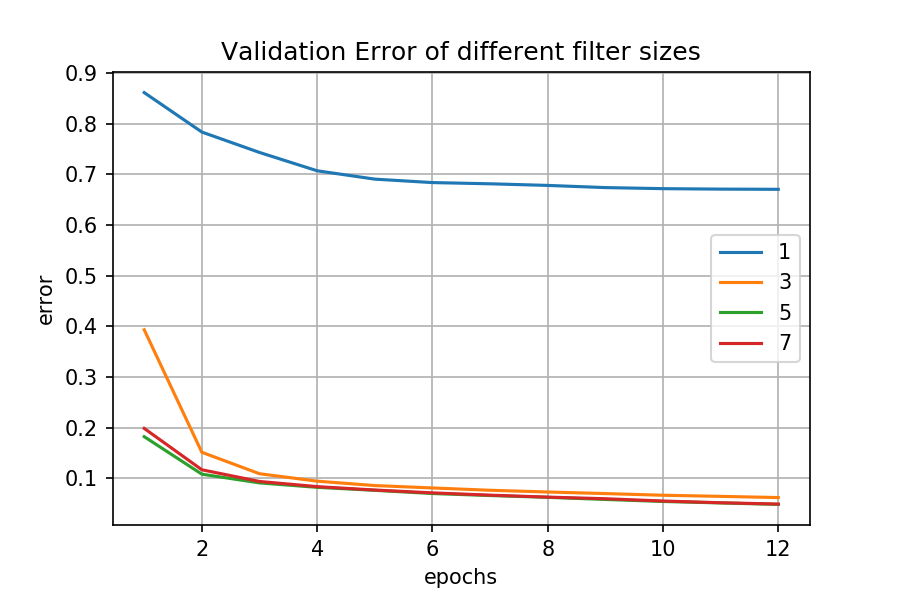
\includegraphics[width=11.70cm, height=7.9cm]{plots/filter/valid_error_12.png}
  \caption{
    \label{fig:filter}
    Change of validation error during 12 training epochs and with different filter sizes in the convolutional layer.
}
\end{figure}


\section{Random Search}\label{rs}

Finally the best configuration of four hyperparameters is found by random search. The following hyperparameters and values are tested:

\begin{itemize}
	\item learning rate $\in [10^{-4}, 10^{-1}] $
	\item batch size $\in [16, 128]$
	\item number of filters $\in [2^{3}, 2^{6}]$
	\item filter size $\in \{3, 5\}$
\end{itemize}

Each random configuration has a budget of 6 epochs and in total 50 configurations (iterations) are tested. HpBandster is used for implementation.\\
\autoref{fig:rs_all} shows the validation error of the configurations during 50 iterations of random search. Here you see that the best configuration is already found in the first iteration. It was the following: batch size: 23, number of filters: 38, filter size: 5, learning rate: 0.058781359070765656.\\
\autoref{fig:rs_best} shows the validation error of the best configuration during 12 epochs. Here you see small jumps in the error. The trained network with the best configuration achieved a test error of 4.3\% on unseen test data. 


\begin{figure}[H]
	\centering 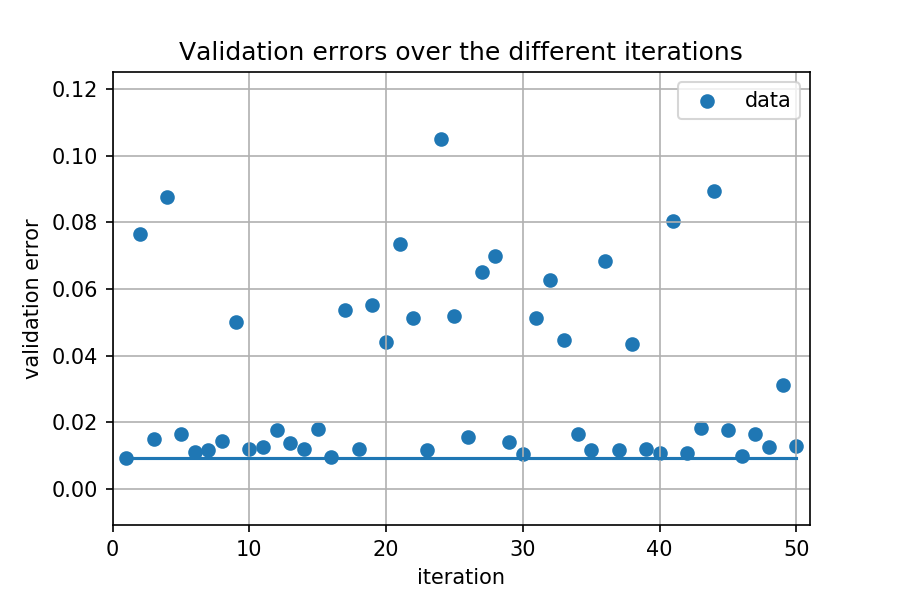
\includegraphics[width=11.70cm, height=7.9cm]{plots/rs/random_search.png}
	\caption{
		\label{fig:rs_all}
		Validation errors of the 50 tested configurations evaluated during 6 epochs. 
	}
\end{figure}

\begin{figure}[H]
	\centering 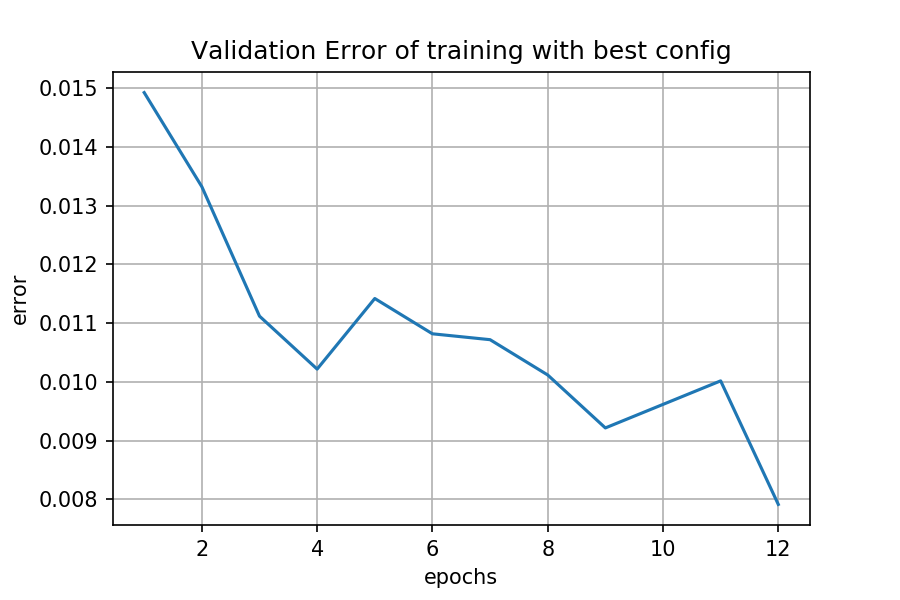
\includegraphics[width=11.70cm, height=7.9cm]{plots/rs/valid_error_12.png}
	\caption{
		\label{fig:rs_best}
		Change of validation error during 12 training epochs with the best find configuration during random search.
	}
\end{figure}

\section{Conclusion}

With this exercise you see that hyperparameter tuning is important for the network performance. So with the right values the error converges faster and this could lead to better learning. Random Search is a good method to test different configuration in short time.


%\begin{itemize}
%	\item learning rate: 0.15
%	\item epochs: 30
%	\item batch size: 30
%	\item optimizer: stochastic gradient descent
%\end{itemize}

%\autoref{fig:train_valid_error}


\end{document}
